\documentclass{article}
\usepackage[margin=0.8in]{geometry}
\usepackage{amsmath}
\usepackage{ctex}
\usepackage{siunitx}
\usepackage{multirow}
\usepackage{bigstrut}
\usepackage{graphicx}
\usepackage{hyperref} 
\title{声速测量实验报告}
\author{姓名:宋建宏\,\, 学号:PB21020677\,\, 班级:203院22级5班\\ 日期:2023年4月7日}
\date{}

\begin{document}
\maketitle

\section*{实验目的}
用共振干涉法和相位比较法测量气体、液体中的声速;用时差法测量固体中的声速;学习示波器的调试和使用,练习线性拟合的数据处理方法。

\section*{实验原理}
声波是一种机械波,其在理想气体中的传播速度 $v$ 满足
    \begin{equation}\label{lixiang}
        v=\sqrt{\frac{\gamma R T}{M}}
    \end{equation}
其中 $\gamma=C_p / C_V$ 是比热容比、 $R$ 为普适气体常量、 $M$ 为气体的摩尔质量、 $T$ 为气体的热力学温度。
如果忽略空气中的水蒸气和其他夹杂物的影响,在 $\SI{0}{\degreeCelsius}(T_0 =\SI{273.15 }{K},\,p = \SI{101.3}{kPa})$时干燥的理想空
气的声速为 $v_0=331.45 \mathrm{~m} / \mathrm{s}$, 在摄氏温度 $t$ 下声速的公式为
\begin{equation}\label{shengsu}
        v_t=v_0 \sqrt{1+\frac{t}{273.15}}
    \end{equation}
声波参数(波速 $v$, 波长 $\lambda$ ,频率 $f$ )之间满足
\begin{equation}\label{eq1}
    v=\lambda f
\end{equation}
因此可通过测定声波的波长和频率来求声速。 声波的频率 $f$ 等于声源的电激发
信号频率, 由低频信号发生器上的频率直接给出。声波的波长可用共振干涉法
(驻波假设下)和相位比较法(行波近似下)来测量。本实验用前者测量空气中的声速,
用后者测量液体(水)中的声速。

\subsection*{谐振频率的测量原理}
在S1和S2之间保持一定间距的情况下, 观察接收波的电压幅度变化, 调节正弦信号
频率, 当在某一频率点处电压幅度最大时, 此频率即为压电换能器 $S1,S2$ 的相匹配
频率点, 记下该谐振频率$f$。实际操作时从频率最大位开始调节,每一位都要满足电压幅度最大, 依次调节到最小位, 结果即为谐振频率。

注意: 当换能器发射面 S1 和接收面 S2 保持平行时才有较好的接收效果。为了得到较清盺的接收波形, 需要将外加的驱动信号频率调节到发射换能器 S1 谐振频率点 $f$ 处, 才能较好地进行声能与电能的相互转 换, 以提高测量精度, 得到较好的实验效果。

\subsection*{共振干涉法原理}
实验装置如图, 当S2的接收表面直径较大时,将会反射部分和声源同频率的声波。
入射波和反射波振动方向与频率相同而发生相干叠加,当S1 和 S2 相互平行
时且接收器位置固定时, S1 前进波和 S2 反射波在 S1 和 S2 之间
往返反射, 相互干涉叠加, 发生共振, 形成驻波, 声场中将会形成稳定的强度分布,
在示波器上观察到的是这两个相干波在S2处合成振动的情况。

在驻波场中, 空气质点位移的图像不能直接观察到, 可以通过仪器观测声压
(空气中由于声扰动而引 起的超出静态大气压强的那部分压强)来间接反映位移变化。
声场中空气质点位移为波腹的地方, 声压最小; 位移为波节的地方, 声压最大。
如图所示。当发生共振时,接收器S2反射端面位置近似为振幅的波节,
即声压的波腹, 即此处位移为0,接收到的声压信号最强。连续改变距离 $L$,
示波器可观察到声压波幅在最大值和最小值之间呈周期性变化。当S1、S2之间的
距离变化量 $\Delta L$ 为半波长 $\lambda / 2$ 的整数倍时,
$\Delta L=n \cdot \lambda / 2$, 出现稳定的驻波共振现象, 声压最大,
相邻两次声压波幅极大值所对应的距离的变化即为半波长,所以有
$$\Delta L_{n-1}=\left|L_{n+1}-L_1\right|\qquad\lambda_i=\Delta L_{i+2}=\left|L_{i+2}-L_i\right|$$

\subsection*{相位比较法原理}
波不仅传播振幅,也进行相位的传播,沿传播方向上的任意两点,如果其振动状态相同,
则这两点同位相,或者说其位相差为$2\pi$的整数倍,这两点间的距离即为波长的整数倍。

实验装置接线如图所示,置示波器功能于X-Y方式。当S1发出的平面超声波通过媒质到达
接收器S2,发射端S1接示波器的Y输入端,接收器S2接至示波器的X输入端。当发射器与
接收器之间有相相位差,可通过李萨如图形来观察。

移动S2,改变S1和S2之间的距离$L$,相当于改变了发射波和接收波之间的相位差,
示波器上的图形$L$不断变化。当S1、S2之间距离改变半个波长
$\Delta L=\lambda / 2$ 时,$\Delta \varphi=\pi$ 。每当相位差改变
$2 \pi$ 时,示波器中的李萨如图形相应变化一个周期(如图,随着振动的相
位差从$0 \sim \pi$的变化,李萨如图形从斜率为正的直线变为椭圆,再变到
斜率为负的直线)。因此,每移动半个波长,就会重复出现斜率符号相反的直线,
这样就可以测得波长 $\lambda$,根据式$v=\lambda f$即可计算出声音传播的速度。

对于多数空气声速测量装置,发射器频率一定时移动接收器位置,既能看到接收器与
发射器信号等相位现象周期性地出现,也能看到接收器声压极大值信号周期性地出现。
前者的位移平均周期为 $\lambda$,后者为$\lambda/2$。依次测量出一系列等相点
或振楅极值点的位置 $l_i$ (对应序号为 $i$ ),求出直线方程 $l=a+bi$ 的斜率
$b$,求出波长 $\lambda$,进而求出声速。

\subsection*{时差法原理}
本实验用时差法来测定固体(黄铜棒、有机玻璃棒)中的声速。不用以上两种方法是
因为以上两种方法测量声速是用示波器观察波峰和波谷或者观察两个波的相位差,这样
做读数位置不易确定。

实验装置如图,将脉冲调制的电信号加到发射换能器上,声波在媒质中传播,从信号源经过
时间 $t$ 后,到达距离为$L$处的接收换能器,那么可以用$v=L / t$求出声波在
媒质中传播的速度。由于不知道导线以及其他器材的声波路程 (事实上也无法测量),
本实验采用差值法,使用两根不同长度的相同材质的棒,分别测出所用时间,
用$v=\Delta L / \Delta t$ 计算波速。
\newpage

\section*{实验仪器}
\

SV5型声速测量仪、对踪示波器、有机玻璃棒、黄铜棒、游标卡尺。
\section*{测量记录}
谐振频率:$\SI{36840.000}{Hz}$ \ \ \ \ \ \ \ \ \ \   实验温度:$\SI{21.8}{\degreeCelsius}$

各实验测量数据如下:

% Table generated by Excel2LaTeX from sheet 'Sheet1'
\begin{table}[htbp]
    \centering
    \caption{共振干涉法实验数据}
    \begin{tabular}{|l|r|r|r|r|r|r|r|r|r|r|r|r|}
        \hline
        序号              & 1     & 2     & 3     & 4     & 5     & 6     & 7      & 8      & 9      & 10     & 11     & 12 \bigstrut     \\
        \hline
        $L_0/\SI{}{mm}$ & 74.06 & 78.90 & 83.62 & 88.32 & 93.08 & 97.78 & 102.57 & 107.16 & 111.88 & 116.60 & 121.26 & 125.38 \bigstrut \\
        \hline
    \end{tabular}%
\end{table}%
% Table generated by Excel2LaTeX from sheet 'Sheet1'
\begin{table}[htbp]
    \centering
    \caption{相位比较法实验数据}
    \begin{tabular}{|l|r|r|r|r|r|r|r|r|}
        \hline
        序号              & 1     & 2     & 3      & 4      & 5      & 6      & 7      & 8 \bigstrut      \\
        \hline
        $L_i/\SI{}{mm}$ & 76.56 & 96.28 & 117.40 & 137.70 & 157.30 & 177.12 & 196.64 & 217.88 \bigstrut \\
        \hline
    \end{tabular}%
\end{table}%
% Table generated by Excel2LaTeX from sheet 'Sheet1'
\begin{table}[htbp]
    \centering
    \caption{时差法实验数据}
    \begin{tabular}{|l|cc|ccc|}
        \hline
           & \multicolumn{2}{c|}{黄铜棒} & \multicolumn{3}{c|}{有机玻璃棒} \bigstrut                                      \\
        \hline
        序号 & 1                        & 2                                  & 1      & 2      & 3                \\
        \hline
        长度$L/\SI{}{mm}$ & 219.21                   & 259.96                             & 190.80 & 229.98 & 271.80 \bigstrut \\
        \hline
        时间$t/\SI{}{\mu s}$ & 68                       & 80                                 & 115    & 136    & 149 \bigstrut    \\
        \hline
    \end{tabular}%
\end{table}%

\section*{数据处理}
\subsection*{共振干涉法}
使用Origin对数据进行线性拟合,结果如图\ref{graph1}。记序号为$j$,有 
\[L=4.71j+69.48\,(\SI{}{mm})\]
因此波长的测定值为$\SI{9.42}{mm}$。根据式\eqref{eq1}有
\[v=\lambda f=\SI{9.42}{mm}\times \SI{36840}{Hz}=\SI{347.03}{m/s}\]

\begin{figure}[h]
    \centering
    \caption{共振干涉法的拟合图象}
    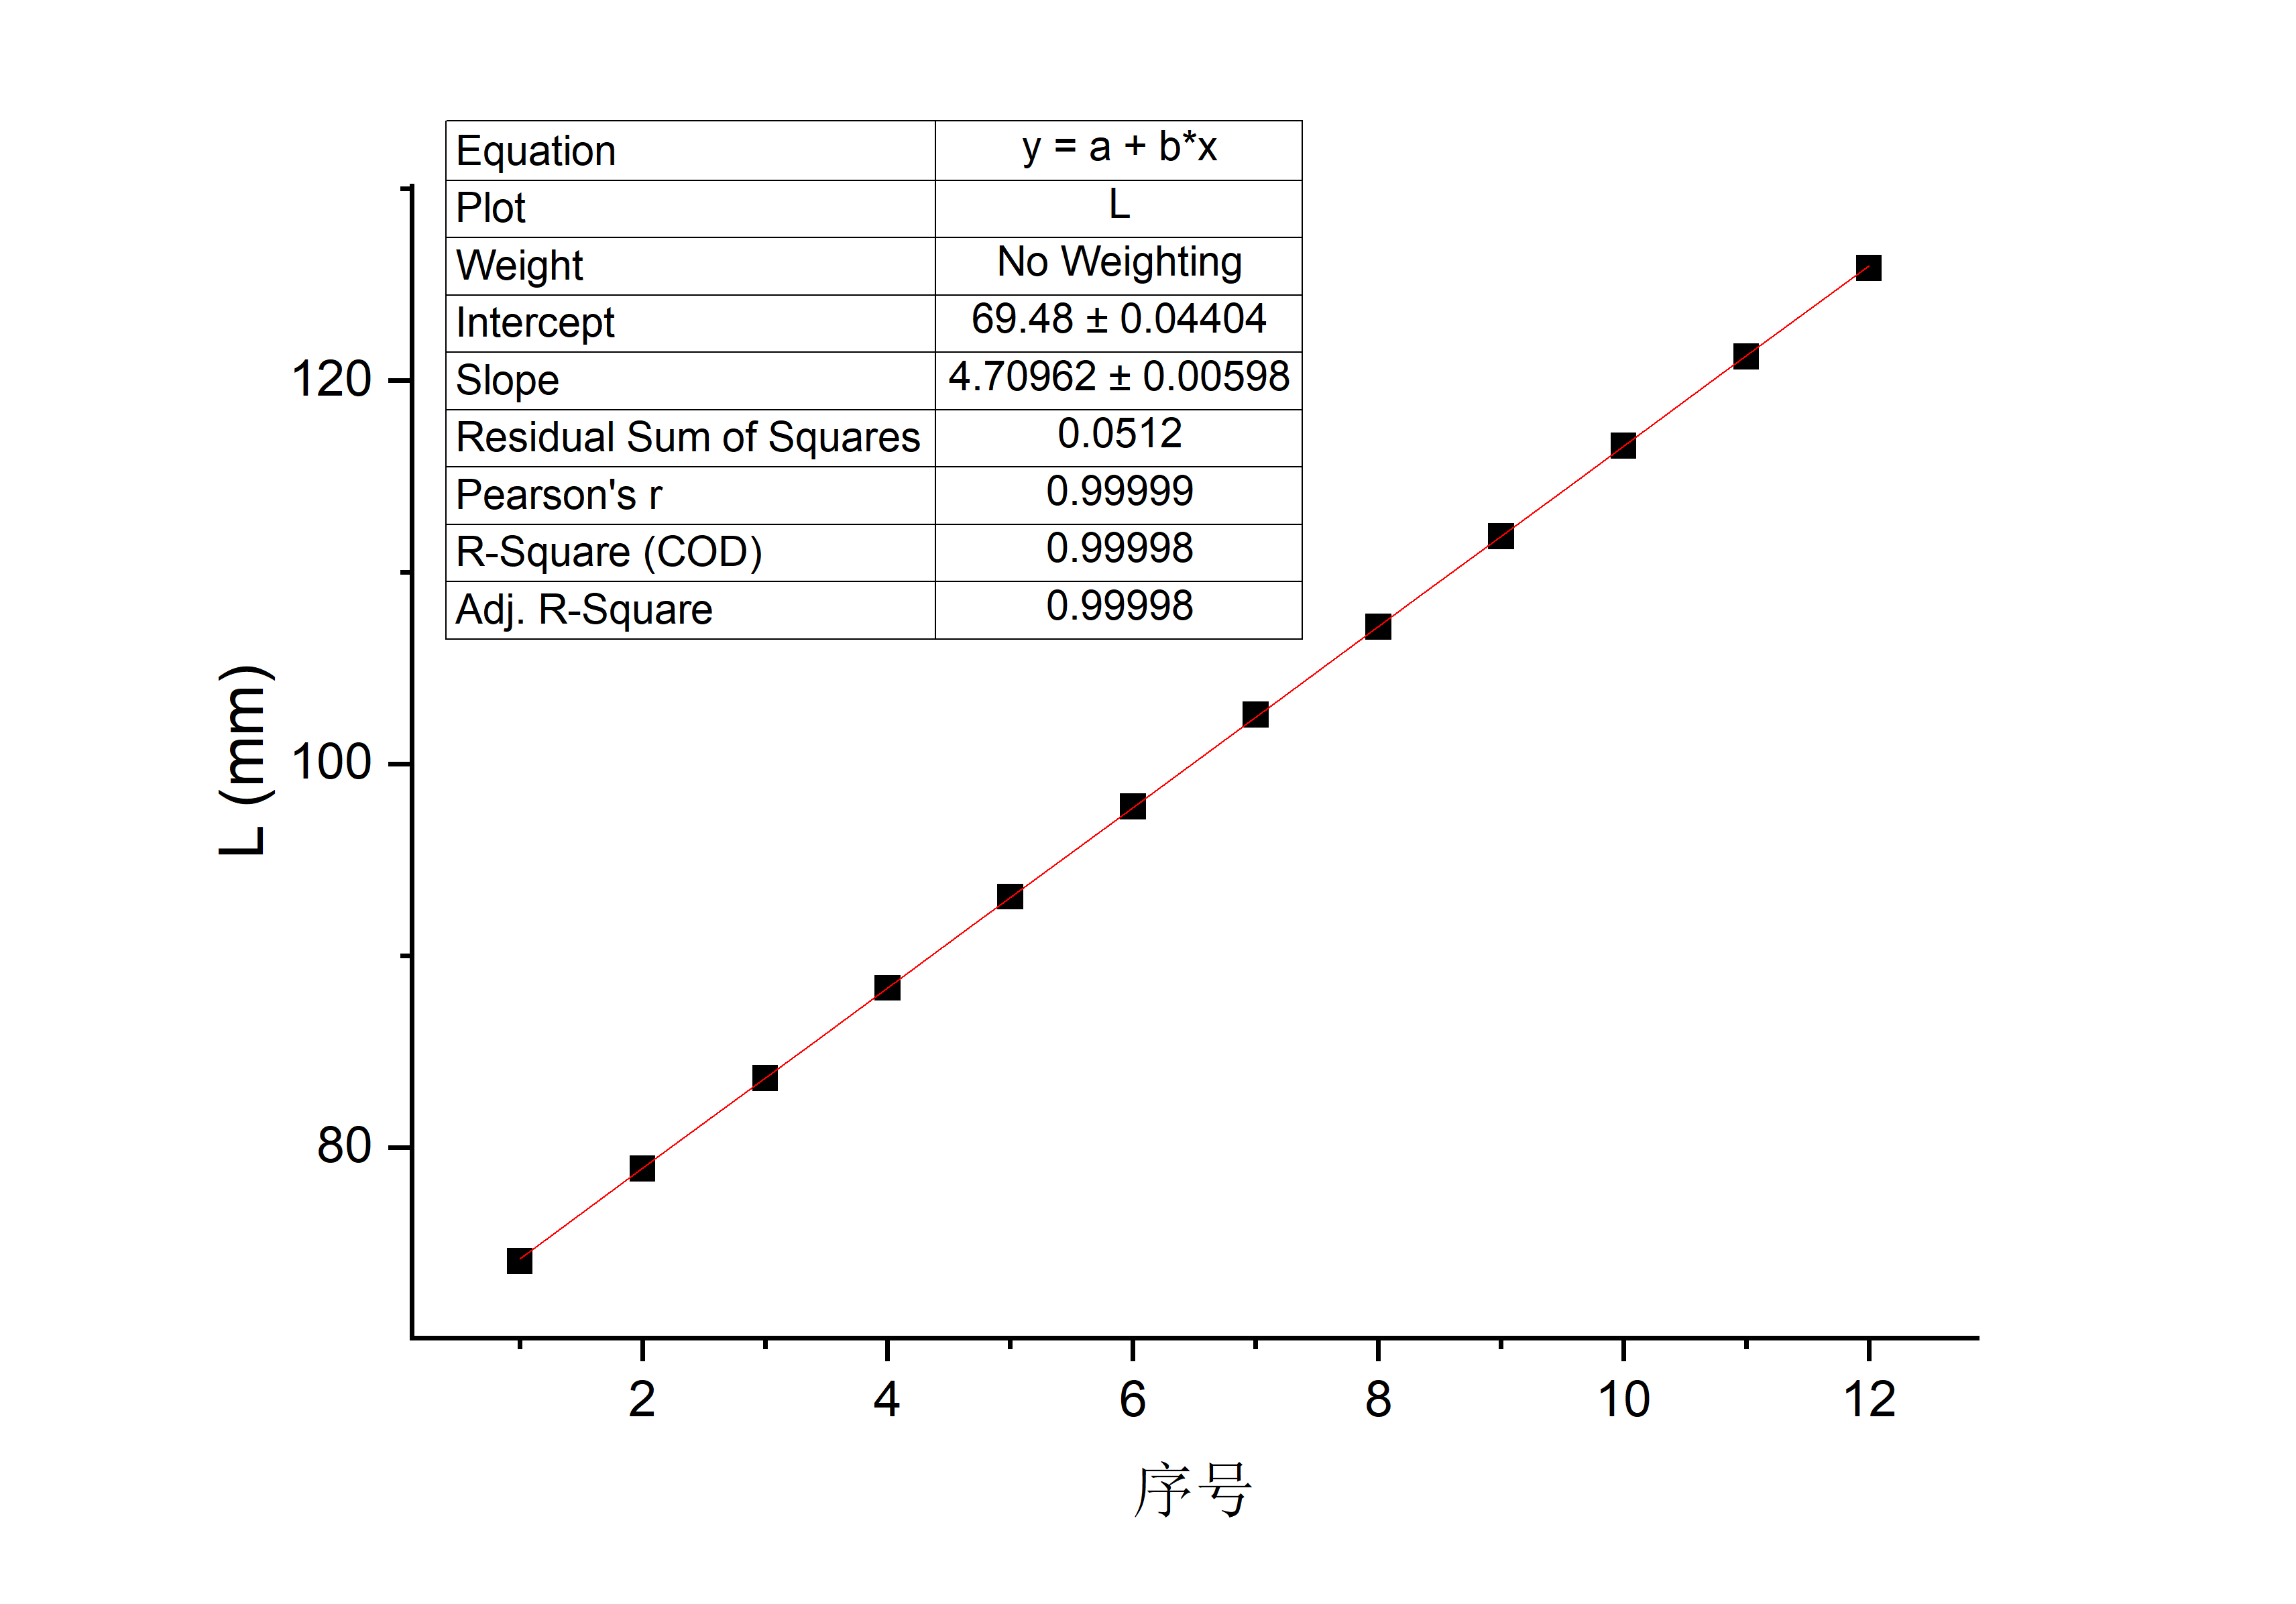
\includegraphics[scale=0.5]{graph1.png}
    \label{graph1}
\end{figure}


\subsubsection*{波长的不确定度}

% Table generated by Excel2LaTeX from sheet 'Sheet1'
\begin{table}[htbp]
    \centering
    \caption{波长的测量列}
      \begin{tabular}{|l|r|r|r|r|r|r|r|r|r|r|}
      \hline
      序号    & 1     & 2     & 3     & 4     & 5     & 6     & 7     & 8     & 9     & 10 \bigstrut\\
      \hline
      $\lambda/\SI{}{mm}$     & 9.56  & 9.42  & 9.46  & 9.46  & 9.49  & 9.38  & 9.31  & 9.44  & 9.38  & 8.78 \bigstrut\\
      \hline
      \end{tabular}%
    \label{tab:addlabel}%
  \end{table}%
  
  
测量列的标准差为 $\sigma=\sqrt{\frac{\sum_{i=1}^{10}\left(\lambda_i-\bar{\lambda}\right)^2}{10-1}}=0.22 \mathrm{~mm}$, 故 $u_{\mathrm{A}}=\frac{\sigma}{\sqrt{10}}=0.07 \mathrm{~mm}$ 。置信概率为 $P=0.95$, 由图可获得的波长测量数据为10个, 则取 $t_{0.95}=2.18$, 因此A类不确定度为 $U_{\mathrm{A}}=t_{0.95} u_{\mathrm{A}}=0.16 \mathrm{~mm}$

仪器(游标卡尺)的最大允差 $\Delta_{\text {仪 }}=0.02 \mathrm{~mm}$, 置信系数 $C=\sqrt{3}$, 估计误差 $\Delta_{\text {估 }}=0.01 \mathrm{~mm}$, 因此 $\Delta_{\mathrm{B}}=\sqrt{\Delta_{\text {仪 }}^2+\Delta_{\text {技 }}^2}=0.02 \mathrm{~mm}$; 取 $k_{0.95}=1.645$, 则 $U_{\mathrm{B}}=k_{0.95} \cdot \frac{\Delta_{\mathrm{B}}}{C}=0.02 \mathrm{~mm}$ 。因此波长的不确定度为 $U_{\lambda, 0.95}=\sqrt{U_{\mathrm{A}}^2+U_{\mathrm{B}}^2}=0.16 \mathrm{~mm}$

\subsubsection*{声速的不确定度}

谐振频率只有B类不确定度。信号发射器的最大允差 $\Delta_{\text {仪 }}=0.001 \mathrm{~Hz}$,置信系数 $C=3$,$k_{0.95}=1.960$,则 $U_{\mathrm{B}}=k_{0.95} \cdot \frac{\Delta_{\mathrm{B}}}{C}=0.0007 \mathrm{~Hz}$ 。因此频率的不确定度为 $U_{f, 0.95}=U_{\mathrm{B}}=0.0007 \mathrm{~Hz}$

由不确定度的传递公式, $U_v=v \sqrt{\left(\frac{U_\lambda}{\lambda}\right)^2+\left(\frac{U_f}{f}\right)^2}=\SI{6}{m/s}$ 。
因此本实验的最终结果应表示为

$$
    v=(347 \pm 6) \mathrm{m} / \mathrm{s}\quad( P=0.95)
$$
\subsubsection*{误差分析}
由式\eqref{shengsu}得实验温度下声速的理论值为 $v_s=344.4 \mathrm{~m} / \mathrm{s}$, 因此本实验的相对误差为
$$
    \delta=\frac{\left|v-v_s\right|}{v_s}=0.08\%
$$
可见本实验的误差是比较小的, 在实验过程中有以下因素引起误差:
\begin{enumerate}
    \item 在观察示波器寻找振幅最大值时, 为了避免回程差旋转把只能单向扭动, 这导致当实验者观察到振幅最大值出现时 $L$ 事实上已经超过了, 这引起了误差;
    \item 游标卡尺的读数误差。
\end{enumerate}


\subsection*{相位比较法}
使用Origin对数据进行线性拟合,结果如图\ref{graph2}。记序号为$i$,有 
\[L=20.17i+56.58\,(\SI{}{mm})\]
因此波长的测定值为$\SI{40.34}{mm}$。根据式\eqref{eq1}有
\[v=\lambda f=\SI{40.34}{mm}\times \SI{36840}{Hz}=\SI{1471.60}{m/s}\]


\begin{figure}[h]
    \centering
    \caption{相位比较法的拟合图象}
    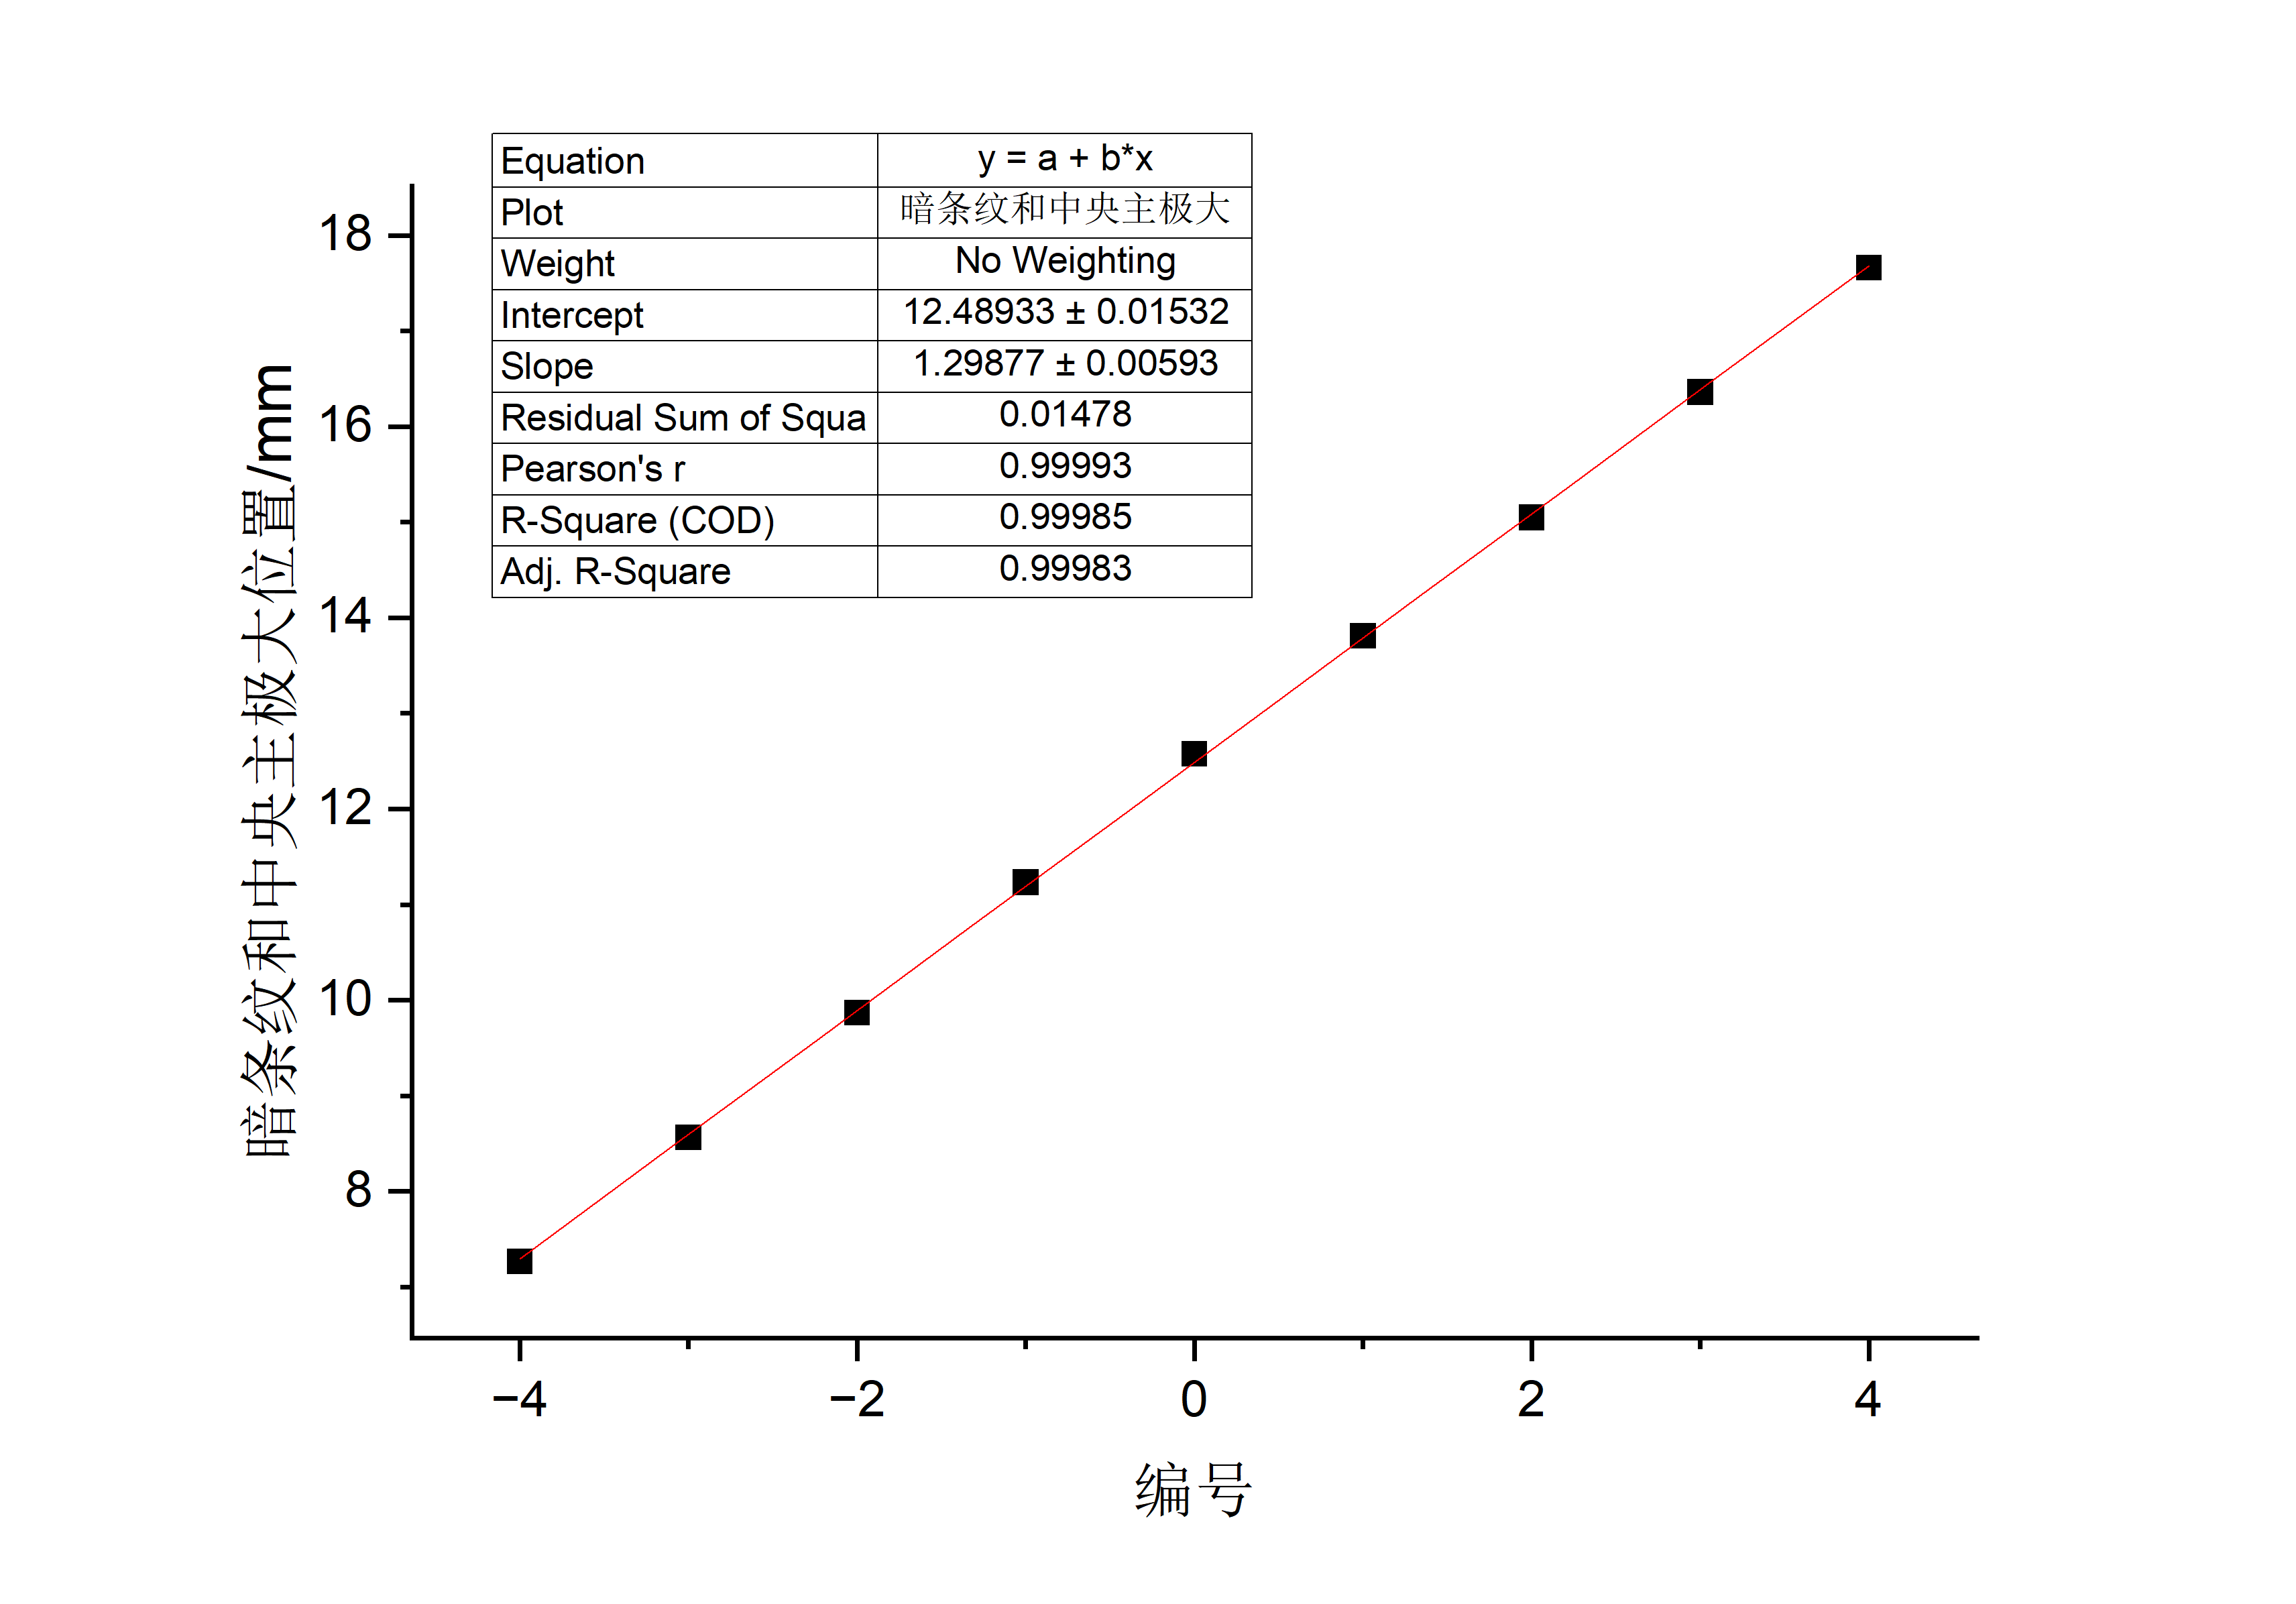
\includegraphics[scale=0.5]{graph2.png}
    \label{graph2}
\end{figure}
\subsubsection*{误差分析}
查资料知实验温度下水中声速大约为 $v_s=1497 \mathrm{~m} / \mathrm{s}$, 因此本实验的相对误差约为
$$
    \delta=\frac{\left|v-v_s\right|}{v_s}=0.17 \%
$$
可见本实验的误差是比较小的, 在实验过程中有以下因素引起误差:
\begin{enumerate}
\item 实验用液体不是纯水,会导致误差以及不确定度的产生;
\item 在观察示波器时,人眼不能精确地确定直线;
\item 为避免回程差只能单向转动;
\item 游标卡尺的读数误差。
\end{enumerate}


\subsection*{时差法}
对于黄铜棒,我们有$\Delta L=\SI{40.75}{mm}$,$\Delta t=\SI{12}{\mu s}$,故可得黄铜棒的声速
\[v=\frac{\Delta L}{\Delta t}=\SI{3395.83}{m/s}\]

对于有机玻璃棒,通过最小二乘法拟合,我们得到
\[L=2.3332t-48.504(\si{}{mm})\]
即\[v=\SI{2333.2}{m/s}\]

\subsubsection*{误差分析}
由于缺少实验温度下黄铜棒、有机玻璃棒中声速的标准值,因此无法计算相对误差。

由于有机玻璃棒有三组数据,线性相关系数$r^2=0.97652$,据此可推测测量结果可信度较高。

而测黄铜棒声速的实验由于只有两种长度的棒,因此只能得出一组数据,数据
的偶然性较大,综合来说无法估算可信度。

在实验过程中有以下因素引起误差:
\begin{enumerate}
    \item 实验用的黄铜棒、有机玻璃棒化学组分不确定,而且不同的黄铜棒、有机玻璃棒所含杂质以及杂质
    的分布也不相同,会导致误差以及不确定度的产生;
    \item 每个棒两端涂抹的润滑油的量和螺栓的长度形状等具有随机性,因此对最终的测定值有一定的影响;
    \item 测量时间的仪器精度不够, 分度值为 $\SI{1}{\mu s}$,其误差体现在计算结果上就是$10^3$量级的误差;
    \item  游标卡尺的读数误差。
\end{enumerate}




\section*{思考题}
\subsection*{定性分析共振法测量时,声压振幅极大值随距离变长而减小的原因。}
声波在实际介质(实验中为干燥空气) 中传播时,由于扩散、吸收和散射等原因,会随着离开
声源的距离增加而逐渐减弱。振幅的大小表示波动能量的大小,声波在传播过程中的能量损失就通
过声压振幅的极大值减小表现出来。

声波在传播过程中的减弱现象与传播距离、声波频率和界面等因素有关。由于接收器的反射面
不是理想的刚性平面,它对入射声波能量也有吸收。实验使用的声波频率较高,频率越高的声波在
传播过程中更容易受空气影响,因此在传播路程增加时能量损失的现象更为明显。
\subsection*{声速测量中驻波法、相位法、时差法有何异同?}
不同点:
\begin{enumerate}
    \item 从波源方面说, 驻波法、相位法用的是连续正弦波,而时差法用的是脉冲波.
    \item 从测量仪器方面说, 驻波法、相位法要用到示波器,而时差法直接使用波源测量。
    \item 从实验操作方面说, 驻波法、相位法、时差法三者所用到的记录数据方法各不相同。 驻波法
    是通过观察声压振幅达到最大值;相位法是通过观察李萨如图形的周期性变化;时差法是直
    接观察信号发生器上的时间显示。
\end{enumerate}

相同点:
\begin{enumerate}
    \item 从波源方面说,驻波法、相位法用的都是连续波。
    \item 从测量仪器方面说,驻波法、相位法都要用示波器、游标卡尺和 SV5 型声速测量仪。
    \item 从原理方面说,驻波法、相位法所利用的原理相同,均是发射波和返回波形成驻波, 测出波长
    后乘以谐振频率来计算波速。
\end{enumerate}
\subsection*{各种气体中的声速是否相同,为什么?}
不同气体中的声速一般不同,通过理想气体中声速的计算式\eqref{lixiang}可知,理想气体中声速与气体的比
热容比、摩尔质量有关,这是由气体的性质决定的。其次,由于湿度对声速也有影响,对相同化学构
成的气体,在湿度不同的情况下,其中声速也会不相同。
\end{document}